\documentclass[12pt,a4paper]{article}
\usepackage[utf8]{inputenc}
\usepackage[russian]{babel}
\usepackage[OT1]{fontenc}
\usepackage{amsmath}
\usepackage{amsfonts}
\usepackage{amssymb}
\usepackage{graphicx}
\graphicspath{{Images/}}
\usepackage[left=2cm,right=2cm,top=2cm,bottom=2cm]{geometry}
\usepackage{calc}
\usepackage{wrapfig}
\usepackage{setspace}
\usepackage{indentfirst}
\usepackage{amssymb}
\usepackage{subfigure}
\usepackage{multirow}

\title{
Отчет о выполнении лабораторной работы 3.2.5
Вынужденные колебания в электрическом контуре

}

\author{Комкин Михаил, группа Б01-303}
\newpage
\begin{document}

\maketitle

\textbf{Цель работы:} : исследование вынужденных колебаний и процессов их установления в колебательном контуре.


\textbf{В работе используются:} генератор звуковых частот, вольтметр, частотомер, конденсатор, катушка индуктивности, магазин сопротивлений, осциллограф, универсальный измеритель импеданса.
В работе исследуются колебания, возникающие в параллельном электрическом контуре под действием внешней ЭДС, гармонически меняющейся во времени.\\
\section{Теория}


\begin{figure}[h!]
	\begin{center}
		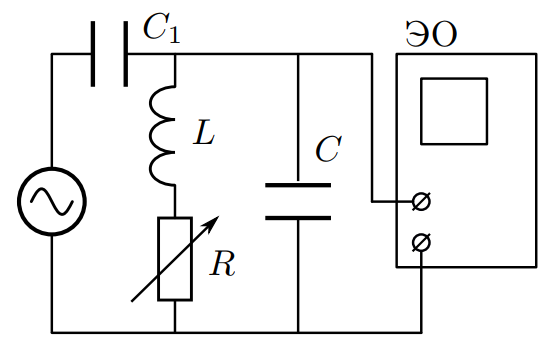
\includegraphics[width = 0.7\textwidth]{ust.png}
		\caption{Схема установки}
		\label{fig:facility}
	\end{center}
\end{figure}

При подключении к контуру внешнего синусоидального источника в
нём возникают колебания, которые можно представить как суперпозицию двух синусоид (2.87): первая — с частотой собственных колебаний
контура и амплитудой, экспоненциально убывающей со временем; вторая — с частотой внешнего источника и постоянной амплитудой. Со временем собственные колебания затухают, и в контуре устанавливаются
вынужденные колебания. Амплитуда этих колебаний максимальна при
резонансе: совпадении или достаточной близости частоты внешнего сигнала и собственной частоты контура. Зависимость амплитуды установившихся колебаний от частоты внешнего сигнала называется резонансной
кривой.

\textbf{Резонансная кривая колебательного контура}
Для экспериментального исследования резонансной кривой тока в параллельном колебательном контуре используется схема, представленная на рис. 1. 

1. Синусоидальный сигнал с генератора подаётся на параллельный колебательный контур через небольшую разделительную ёмкость \(C_1\). Напряжение с конденсатора контура \(C\) поступает на вертикальный вход электронного осциллографа (ЭО). Для регистрации резонансной кривой необходимо, чтобы модули импедансов возбуждающей \(Z_{\text{вх}}\) и измеряющей \(Z_{\text{изм}}\) цепей намного превосходили модуль импеданса самого контура вблизи резонанса \(Z_{\text{рез}} = L / RC\). С этой целью разделительная ёмкость \(C_1\) выбирается настолько малой, что в рабочем диапазоне частот модуль её импеданса \(|Z_{C_1}| = 1/(\omega C_1)\) намного больше модуля импеданса контура на частоте \(\omega\).

Таким образом, амплитуда тока в цепи генератора определяется импедансом \(|Z_{C_1}|\). Эта амплитуда относительно мало меняется в пределах резонансной кривой колебательного контура, что, однако, приводит к некоторому искажению последней по сравнению со случаем, рассмотренным в п. 3.2, где в качестве генератора предполагается источник тока, обладающий большим и постоянным внутренним сопротивлением во всём исследуемом частотном диапазоне. Входное сопротивление осциллографа (измерительной цепи) достаточно велико: \(Z_{\text{изм}} \approx 1\ \text{МОм}\), поэтому его влиянием можно пренебречь.

Указанные ограничения представляются в виде следующих соотношений:
\[
|Z_{C_1}| = \frac{1}{\omega C_1} \gg |Z|_{\text{рез}} = \frac{Q}{\omega_0 C}, \quad R_{\omega} \ll \frac{\omega L}{Q},
\]
где \(\omega_0 = 1/\sqrt{LC}\) — собственная частота контура, а его добротность \(Q = Q_m = \frac{1}{R} \sqrt{\frac{L}{C}}\).

По полученной в эксперименте резонансной кривой \(I_C(\omega)\), представляющей отклик системы — параллельного колебательного контура — на внешнее воздействие, которым является ток генератора \(I_{\omega}\), можно определить его резонансную частоту \(\omega_m \approx \omega_0\) и его добротность \(Q\). При высокой добротности контура частота \(\omega_0\) будет шириной кривой с максимумом резонансной кривой, а добротность будет определяться её относительной шириной: \(Q \approx \omega_0 / \delta \omega\) (см. (2.77)).



Для установления более точной аналитической связи воспользуемся
методом комплексных амплитуд. С учётом условий (1) исследуемая в работе схема эквивалента рассмотренному в п. 3.2 случаю резонанса в \textit{параллельном} контуре. Вычислив модуль из первой формулы (2.78), можно получить следующее выражение для резонансной кривой:
\[
I_C(\omega) = I(\omega) \sqrt{\frac{1 + Q_m^2(\omega/\omega_0 - \omega_0/\omega)^2}{1 + Q_m^2(\omega/\omega_0 - \omega_0/\omega)^2}}. \tag{2}
\]

Из соотношения (2) следует, что на собственной частоте \(\omega_0\) ток в \textit{высокодобротном} контуре почти в \(Q \gg 1\) раз превосходит ток во внешней цепи. Именно по этой причине резонанс в параллельном контуре называется \textit{резонансом токов}.

Как уже отмечалось, резонанс, то есть максимальный отклик на внешнее воздействие, достигается в данной схеме на частоте \(\omega_m\), несколько отличной от собственной \(\omega_0\), в чём можно убедиться при более детальном анализе подкоренного выражения в (2) (см. подробнее п. 3.2 Введения). Дополнительное смещение резонансной частоты и уменьшение добротности контура связаны с шунтирующим действием генератора, приводящим к зависимости амплитуды тока \(I\) от частоты \(\omega\), если его внутреннее сопротивление не достаточно велико. Указанные изменения частоты и гибели добротности контура легко регистрируется в эксперименте.

\subsection*{B. Процессы установления и затухания колебаний в контуре}

Добротность контура может быть определена разными способами, например, по скорости нарастания амплитуды вынужденных колебаний при резонансе или по скорости затухания свободных колебаний.

\begin{figure}[h!]
    \centering
    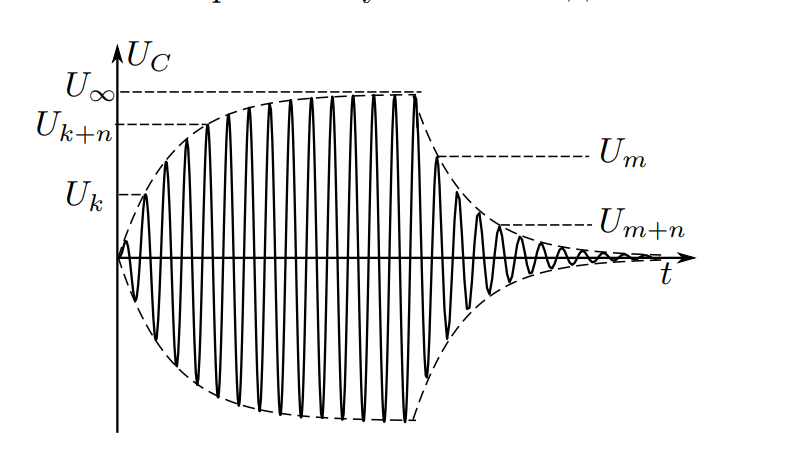
\includegraphics[scale=0.9]{increase.png} % здесь нужно заменить на путь к изображению
    \caption{Нарастание и затухание вынужденных колебаний}
\end{figure}

Нарастание и затухание колебаний (рис. 2) можно наблюдать на экране осциллографа, если подать на контур периодический сигнал с паузами, разделёнными интервалами, в течение которых сигнал отсутствует.
Чем выше добротность Q, тем медленнее нарастают и медленнее затухают колебания в контуре. Получить значение Q можно, измерив логарифмический декремент затухания по скорости нарастания или затухания колебаний. В условиях резонанса огибающая затухающих колебаний
— это «перевёрнутая» огибающая нарастающего участка. Она может быть использована для расчёта логарифмического
декремента затухания по формуле. \\\\
\textbf{Экспериментальная установка}
Схема установки для исследования вынужденных колебаний приведена на рис. 3. Колебательный контур состоит из конденсатора с ёмкостью C, катушки с индуктивностью L и магазина сопротивлений R.
Синусоидальный сигнал генерируется звуковым генератором (ЗГ), а сигнал, состоящий из отрезков синусоиды (цугов), формируется цифровым
генератором электрических сигналов произвольной формы или комбинацией генератора синусоидального сигнала звукового диапазона и электронного реле, прерывающего сигнал с заданной периодичностью. Результирующие сигналы — цуги или непрерывная синусоида — поступают
по отдельным каналам через одинаковые небольшие ёмкости C1 соответственно на клеммы «цуги» и «непр.

\begin{figure}[h!]
	\begin{center}
		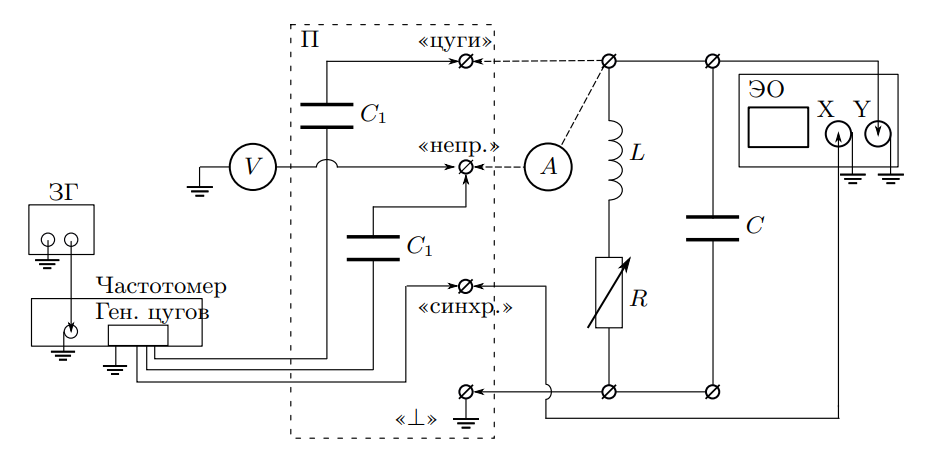
\includegraphics[width = 0.7\textwidth]{ust2.png}
		\caption{Схема установки}
		\label{fig:facility}
	\end{center}
\end{figure}


Эффективное значение тока \( I(\omega) \), текущего к контуру от генератора в режиме непрерывного сигнала, измеряется амперметром \( A \), а соответствующее значение тока в контуре определяется по формуле \( I_C(\omega) = \omega C U_C(\omega) \), где \( U_C(\omega) \) — эффективное напряжение на конденсаторе, измеряемое вольтметром \( V \).

Для визуального наблюдения за процессом колебаний напряжение с ёмкости контура \( C \) подаётся на вход электронного осциллографа. Чтобы картина на экране была устойчивой, частота развёртки осциллографа принудительно синхронизируется с частотой повторения щупов. Для этого на генератор развёртки ЭО подаются следящие с частотой повторения щупов управляющие импульсы, формируемые в блоке электронного реле, клемма «синхр.» которого смонтирована на панели «П».

Используя представленную схему в режиме непрерывного синусоидального сигнала, можно по показаниям приборов и известным параметрам элементов цепи измерить амплитудно-частотную характеристику (резонансную кривую) \( I_C(\omega) \) в необходимом диапазоне частот. Сравнивая результат измерения с теоретической кривой (2), можно определить характеристики колебательного контура \( \omega_m \approx \omega_0 \) и \( Q \).


\end{document}